\chapter{Experimental Evaluation}\label{c:evaluations}



We measured the runtime performance of our privacy\hyp preserving algorithms using the Sharemind secure computing platform.
We instantiated all private aggregators and decision tree classifiers using the SecreC programming language \cite{jagomagis2010secrec} that Sharemind provides.
In Sharemind, the number of the computing parties are restricted by the SMPC protocol that is been used.
Our experiments use the \textit{pd\_shared3p} security protocol, which utilizes three nodes in the private domain.


\textbf{Experimental Setup:}
All experiments were performed on three machines, each running Ubuntu 18.04, using a 2.50 GHz Intel Xeon E5-2670 (v2) system with 4 GBs of memory.

\fixme{Add the correct setup}
% All the time measurements were performed on a 64-bit machine with ten-core Intel Xeon E5-2670 (v2) CPU at 2.50GHz and 4GB of RAM.

\section{Datasets}\label{s:datasets}
As we have stated in section \ref{s:two-types-of-data}, the input data can have many different types, since our system can serve a wide variety of applications.
We have separated the data in two broad categories -- categorical and continuous, therefore our algorithms are also logically separated for those two different kinds of data.

The second reason that we separated our algorithms in those two types, was that we experimented with datasets both types.
In medical research it is common to have standard datasets with continuous exact values corresponding to a set of attributes, but it is also common for the datasets to be semantically annotated.
For instance a dataset of the first form could have a column corresponding to attribute \textit{Height (cm)} with values including $146.84, 139.35, 189.00, 182.68, 160.19, 138.66, 173.06$ etc.
On the other hand, a dataset of the second time would have normalized values including $Tall, Average, Short$ etc.
The synthetic datasets we had available for experimentation were the following.

\textbf{MeSH Dataset:}
MeSH\footnote{\href{https://meshb.nlm.nih.gov/}{https://meshb.nlm.nih.gov/}} provides a hierarchically-organized\footnote{\href{https://meshb.nlm.nih.gov/treeView}{https://meshb.nlm.nih.gov/treeView}} terminology for indexing and cataloging of biomedical information such as MEDLINE/PUBmed and other United States National Library of Medicine (NLM) databases.
Created and updated by the NLM, it is used by articles databases and by NLM's catalog of book holdings.
This dataset is based on the MeSH tree structure.
MeSH terms are represented as normalized values; this means that even attributes like Age, are separated into groups (for instance Child, Adult, etc).
This dataset contains semantically annotated patient data.

\textbf{CVI Dataset:}
Cardiovascular disease is a class of diseases that involve the heart or blood vessels.
Cardiovascular disease includes coronary artery diseases (CAD) such as angina and myocardial infarction (commonly known as a heart attack).
This dataset contains CardioVascular Imaging (CVI) information, which are represented as numerical values – not normalized.

\fixme{Add more...}



\section{Experimental Results}\label{s:results}

\subsection{Histograms}\label{ss:results-histograms}


\begin{figure}[H]
\centering
\centerline{
\begin{minipage}{.5\linewidth}
  \centering
  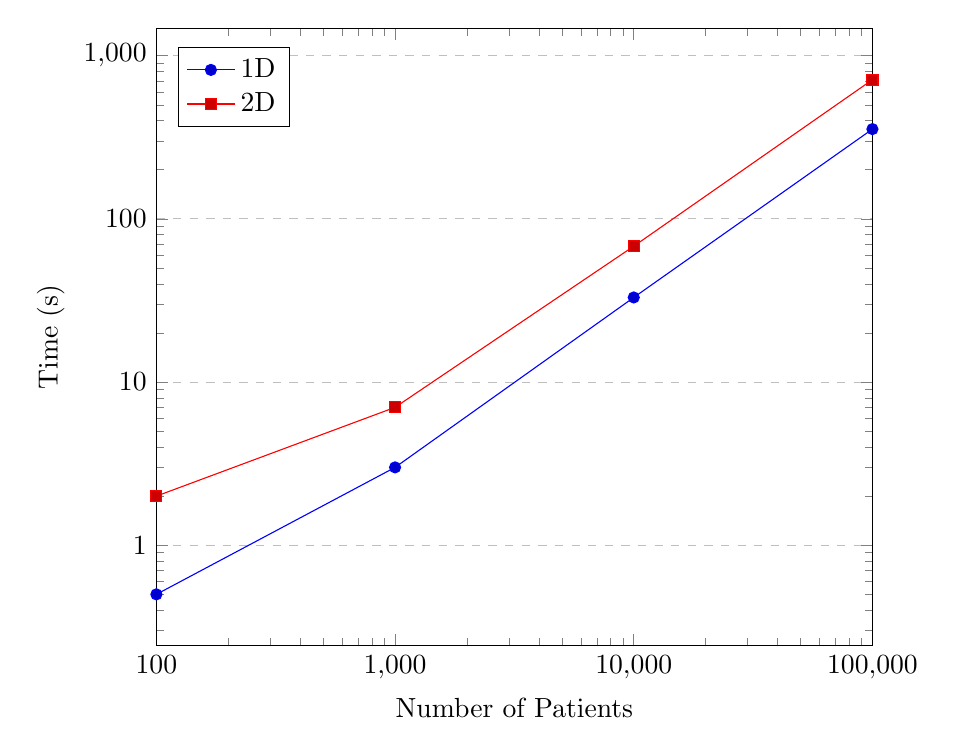
\begin{tikzpicture}
  \begin{axis}[
    legend pos=north west,
    scale only axis,
    enlarge x limits=-1,
    width=\textwidth*0.75,
    ymajorgrids=true,
    xmode=log,
    ymode=log,
    log ticks with fixed point,
    xlabel={Number of Patients},
    ylabel={Time (s)},
    ymin=0,
    grid style=dashed
  ]
  \addplot
    coordinates {(100, 0.5)(1000, 3)(10000, 33)(100000, 355)};
    \addlegendentry{1D}
  \addplot
    coordinates {(100, 2)(1000, 7)(10000, 68)(100000, 713)};
    \addlegendentry{2D}
  \end{axis}
  \end{tikzpicture}
  \caption{Numerical histograms timings}\label{chart:numerical-histogram}
\end{minipage}%
\begin{minipage}{.5\linewidth}
  \centering
  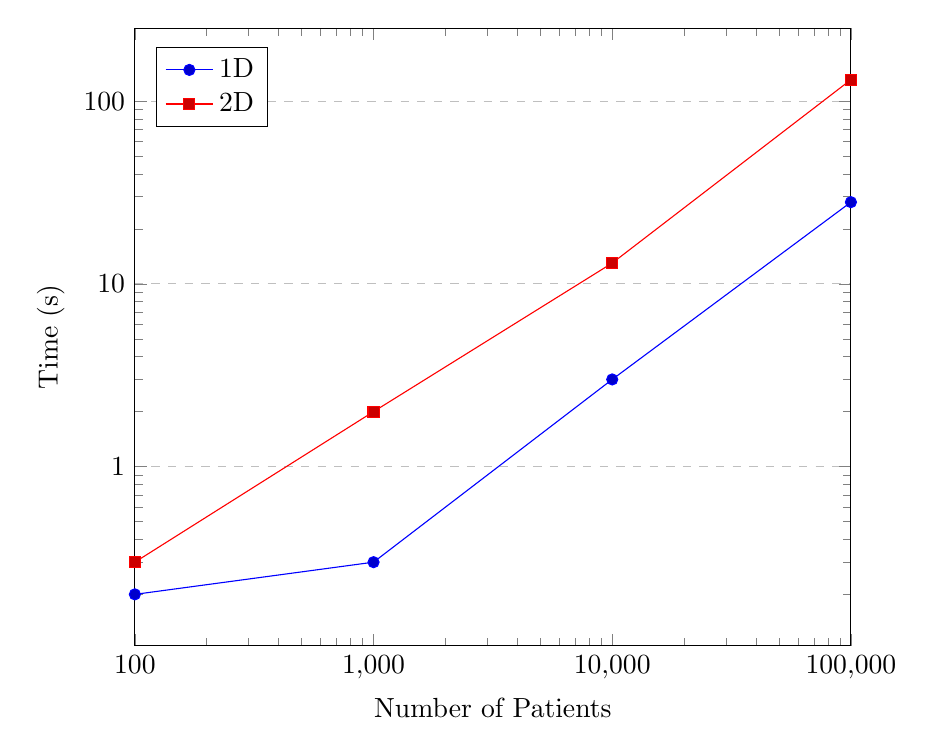
\begin{tikzpicture}
  \begin{axis}[
    legend pos=north west,
    scale only axis,
    enlarge x limits=-1,
    width=\textwidth*0.75,
    ymajorgrids=true,
    xmode=log,
    ymode=log,
    log ticks with fixed point,
    xlabel={Number of Patients},
    ylabel={Time (s)},
    ymin=0,
    grid style=dashed
  ]
  \addplot
    coordinates {(100, 0.2)(1000, 0.3)(10000, 3)(100000, 28)};
    \addlegendentry{1D}
  \addplot
    coordinates {(100, 0.3)(1000, 2)(10000, 13)(100000, 131)};
    \addlegendentry{2D}
  \end{axis}
  \end{tikzpicture}
  \caption{Categorical histograms timings}\label{chart:categorical-histogram}
\end{minipage}
}
\end{figure}


%%%%%%%%%%%%%%%%%%%%%%%%%%%%%%%%%%%%%%%%%%%%%%%%%%%%%%%%%%%%%%%%%%%%%%%%%%%%%%%%%%%

\begin{figure}[H]
\centering
\centerline{
\begin{minipage}{.8\linewidth}
  \centering
  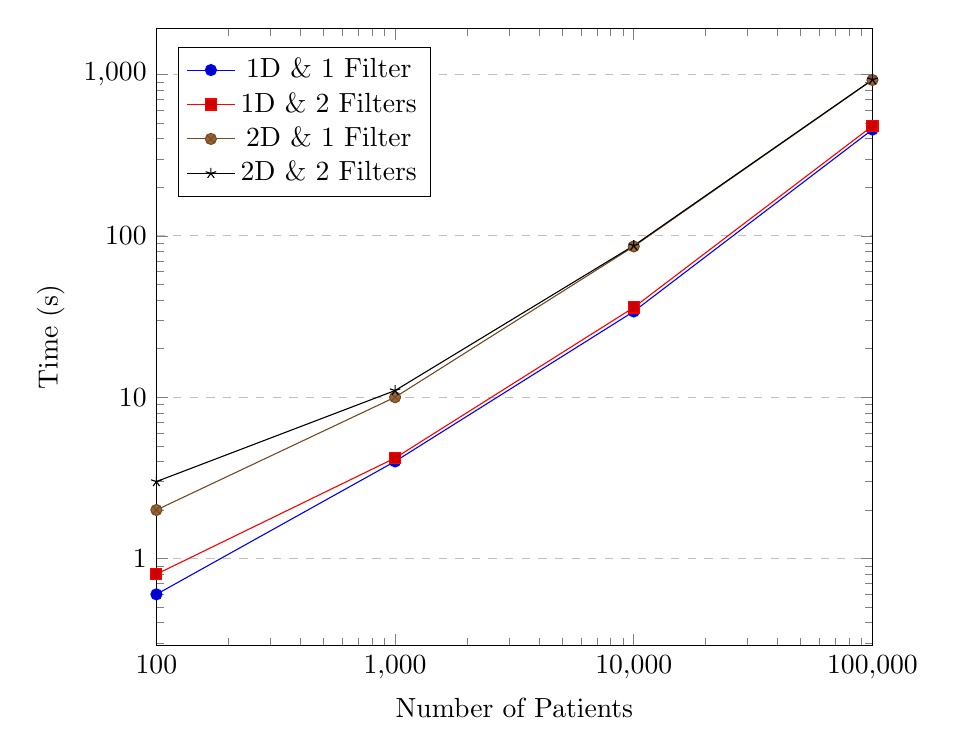
\begin{tikzpicture}
  \begin{axis}[
    legend pos=north west,
    scale only axis,
    enlarge x limits=-1,
    width=\textwidth*0.75,
    ymajorgrids=true,
    xmode=log,
    ymode=log,
    log ticks with fixed point,
    xlabel={Number of Patients},
    ylabel={Time (s)},
    ymin=0,
    grid style=dashed
  ]
  \addplot
    coordinates {(100, 0.6)(1000, 4)(10000, 34)(100000, 456)};
    \addlegendentry{1D \& 1 Filter}
  \addplot
    coordinates {(100, 0.8)(1000, 4.2)(10000, 36)(100000, 480)};
    \addlegendentry{1D \& 2 Filters}
  \addplot
    coordinates {(100, 2)(1000, 10)(10000, 86)(100000, 925)};
    \addlegendentry{2D \& 1 Filter}
  \addplot
    coordinates {(100, 3)(1000, 11)(10000, 87)(100000, 929)};
    \addlegendentry{2D \& 2 Filters}
  \end{axis}
  \end{tikzpicture}
  \caption{Numerical histograms with filters timings}\label{chart:numerical-histogram-filters}
\end{minipage}%
}
\end{figure}


%%%%%%%%%%%%%%%%%%%%%%%%%%%%%%%%%%%%%%%%%%%%%%%%%%%%%%%%%%%%%%%%%%%%%%%%%%%%%%%%%%%
\begin{figure}[H]
\centering
\centerline{
\begin{minipage}{.8\linewidth}
  \centering
  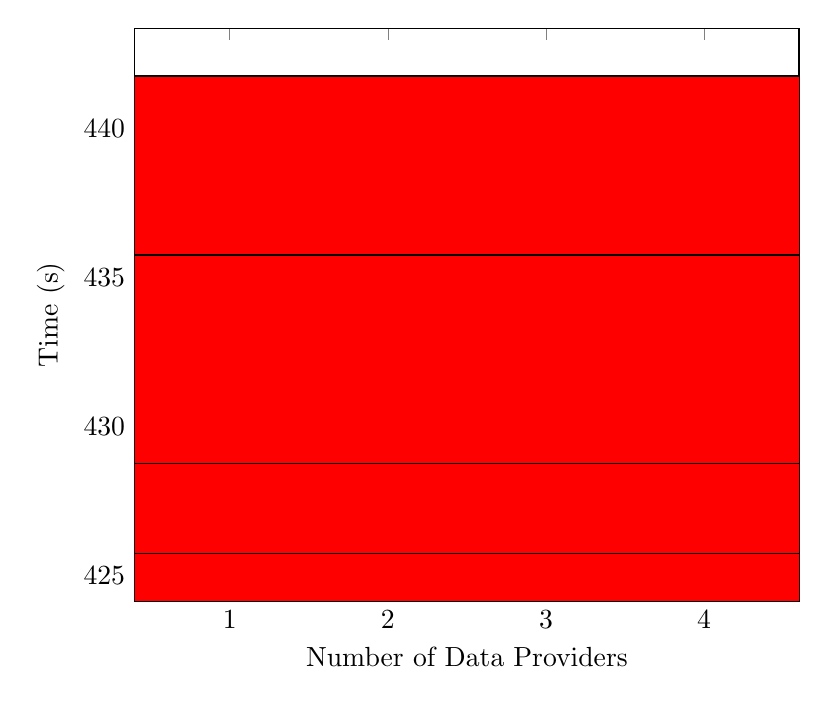
\begin{tikzpicture}
  \begin{axis}[
    legend pos=north west,
    scale only axis,
    ymajorgrids=true,
    xlabel={Number of Data Providers},
    ylabel={Time (s)},
    xtick = {1, 2, 3, 4},
    % ymin = 0,
    grid style=dashed,
    enlarge x limits = 0.2,
    bar width = 40
  ]
  \addplot[ybar, fill=red]
    coordinates {(1, 441.75)(2, 435.75)(3, 428.75)(4, 425.75)};
  \end{axis}
  \end{tikzpicture}
  \caption{Numerical histogram from variable data providers}\label{chart:numerical-histogram-providers}
\end{minipage}%
}
\end{figure}


% \begin{figure}[H]
% \centering
% \centerline{
% \begin{minipage}{.5\linewidth}
%   \centering
%   \begin{tikzpicture}
%   \begin{axis}[
%     legend pos=north west,
%     scale only axis,
%     enlarge x limits=-1,
%     width=\textwidth*0.75,
%     ymajorgrids=true,
%     xmode=log,
%     ymode=log,
%     log ticks with fixed point,
%     xlabel={Number of Patients},
%     ylabel={Time (s)},
%     ymin=0,
%     grid style=dashed
%   ]
%   \addplot
%     coordinates {(100, 5.66)(1000, 10.54)(10000, 57.94)(100000, 536.09)};
%     \addlegendentry{1 data\hyp provider}
%   \addplot
%     coordinates {(100, 54.29)(1000, 56.5)(10000, 75.95)(100000, 267.7)};
%     \addlegendentry{2 data\hyp providers}
%   \addplot
%     coordinates {(100, 54.29)(1000, 56.5)(10000, 75.95)(100000, 267.7)};
%     \addlegendentry{3 data\hyp providers}
%   \end{axis}
%   \end{tikzpicture}
%   \caption{1-Dimensional numerical histograms timings for different number of data\hyp providers}
% \end{minipage}%
% \begin{minipage}{.5\linewidth}
%   \centering
%   \begin{tikzpicture}
%   \begin{axis}[
%     legend pos=north west,
%     scale only axis,
%     enlarge x limits=-1,
%     width=\textwidth*0.75,
%     ymajorgrids=true,
%     xmode=log,
%     ymode=log,
%     log ticks with fixed point,
%     xlabel={Number of Patients},
%     ylabel={Time (s)},
%     ymin=0,
%     grid style=dashed
%   ]
%   \addplot
%     coordinates {(100, 5.66)(1000, 10.54)(10000, 57.94)(100000, 536.09)};
%     \addlegendentry{1 data\hyp provider}
%   \addplot
%     coordinates {(100, 54.29)(1000, 56.5)(10000, 75.95)(100000, 267.7)};
%     \addlegendentry{2 data\hyp providers}
%   \addplot
%     coordinates {(100, 54.29)(1000, 56.5)(10000, 75.95)(100000, 267.7)};
%     \addlegendentry{3 data\hyp providers}
%   \end{axis}
%   \end{tikzpicture}
%   \caption{2-Dimensional categorical histograms timings for different number of data\hyp providers}
% \end{minipage}
% }
% \end{figure}



%%%%%%%%%%%%%%%%%%%%%%%%%%%%%%%%%%%%%%%%%%%%%%%%%%%%%%%%%%%%%%%%%%%%%%%%%%%%%%%%%%%
%%%%%%%%%%%%%%%%%%%%%%%%%%%%%%%%%%%%%%%%%%%%%%%%%%%%%%%%%%%%%%%%%%%%%%%%%%%%%%%%%%%
%%%%%%%%%%%%%%%%%%%%%%%%%%%%%%%%%%%%%%%%%%%%%%%%%%%%%%%%%%%%%%%%%%%%%%%%%%%%%%%%%%%

\subsection{Decision Trees}\label{ss:results-dtrees}

\begin{figure}[H]
\centering
\centerline{
\begin{minipage}{.8\linewidth}
  \centering
  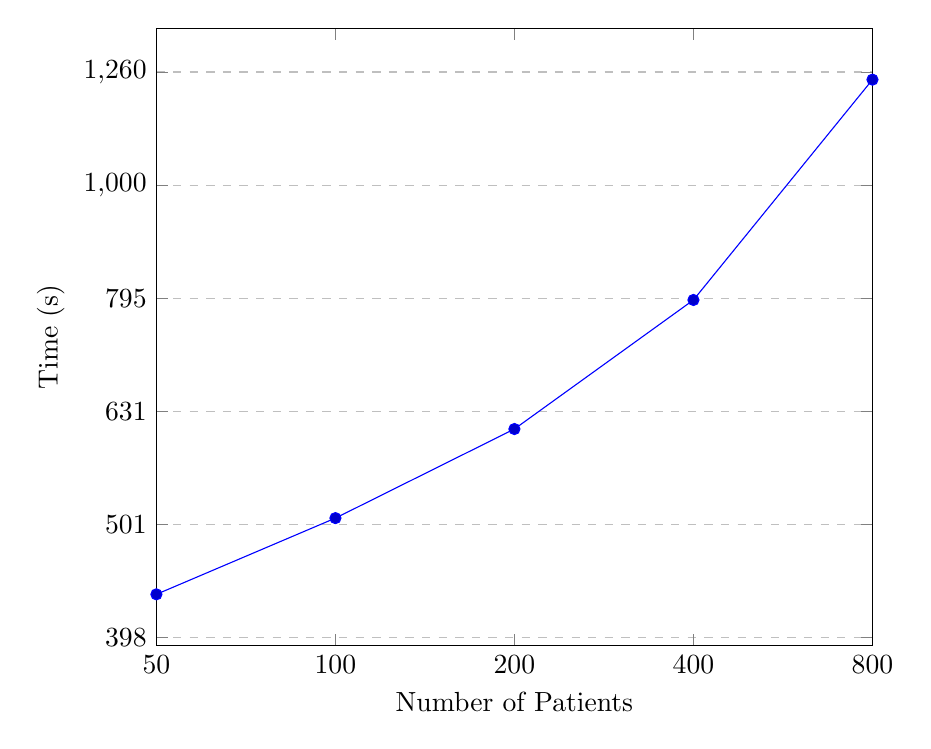
\begin{tikzpicture}
  \begin{axis}[
    legend pos=north west,
    scale only axis,
    enlarge x limits=-1,
    width=\textwidth*0.75,
    ymajorgrids=true,
    xmode=log,
    ymode=log,
    log ticks with fixed point,
    xlabel={Number of Patients},
    xtick = {50, 100, 200, 400, 800},
    ylabel={Time (s)},
    % ymin=0,
    log ticks with fixed point,
    grid style=dashed
  ]
  \addplot
    coordinates {(50, 435)(100, 508)(200, 609)(400, 792)(800, 1240)};
  \end{axis}
  \end{tikzpicture}
  \caption{ID3 decision tree classifier timings with variable patients}\label{chart:id3-patients}
\end{minipage}%
}
\end{figure}

\begin{figure}[H]
\centering
\centerline{
\begin{minipage}{.8\linewidth}
  \centering
  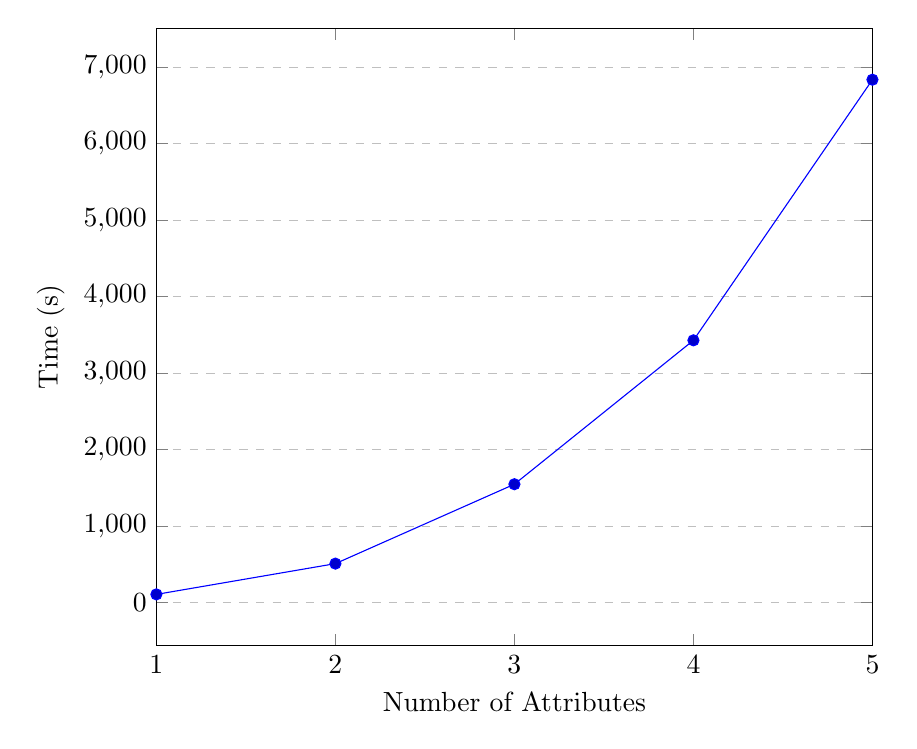
\begin{tikzpicture}
  \begin{axis}[
    legend pos=north west,
    scale only axis,
    enlarge x limits=-1,
    width=\textwidth*0.75,
    ymajorgrids=true,
    log ticks with fixed point,
    xlabel={Number of Attributes},
    xtick = {1, 2, 3, 4, 5},
    ylabel={Time (s)},
    % ymin=0,
    log ticks with fixed point,
    grid style=dashed
  ]
  \addplot
    coordinates {(1, 107)(2, 509)(3, 1547)(4, 3428)(5, 6835)};
  \end{axis}
  \end{tikzpicture}
  \caption{ID3 decision tree classifier timings with variable attributes}\label{chart:id3-attributes}
\end{minipage}%
}
\end{figure}



%
%
% \begin{figure}[H]
% \centering
% \centerline{
% \begin{minipage}{.5\linewidth}
%   \centering
%   \begin{tikzpicture}
%   \begin{axis}[
%     legend pos=north west,
%     scale only axis,
%     enlarge x limits=-1,
%     width=\textwidth*0.75,
%     ymajorgrids=true,
%     xmode=log,
%     ymode=log,
%     log ticks with fixed point,
%     xlabel={Number of Patients},
%     ylabel={Time (s)},
%     ymin=0,
%     grid style=dashed
%   ]
%   \addplot
%     coordinates {(100, 0.548186)(1000, 5.381935)(10000, 52.661779)(100000, 530.589239)};
%     \addlegendentry{Num. ID3}
%   \addplot
%     coordinates {(100, 0.237847)(1000, 2.117192)(10000, 21.845599)(100000, 215.412621)};
%     \addlegendentry{Cat. ID3}
%   \addplot
%     coordinates {(100, 0.548186)(1000, 5.381935)(10000, 52.661779)(100000, 530.589239)};
%     \addlegendentry{Num. C4.5}
%   \addplot
%     coordinates {(100, 0.237847)(1000, 2.117192)(10000, 21.845599)(100000, 215.412621)};
%     \addlegendentry{Cat. C4.5}
%   \end{axis}
%   \end{tikzpicture}
%   \caption{ID3 \& C4.5 decision tree classifier timings for 3 attributes}
% \end{minipage}%
% \begin{minipage}{.5\linewidth}
%   \centering
%   \begin{tikzpicture}
%   \begin{axis}[
%     legend pos=north west,
%     scale only axis,
%     enlarge x limits=-1,
%     width=\textwidth*0.75,
%     ymajorgrids=true,
%     xmode=log,
%     ymode=log,
%     log ticks with fixed point,
%     xlabel={Number of Patients},
%     ylabel={Time (s)},
%     ymin=0,
%     grid style=dashed
%   ]
%   \addplot
%     coordinates {(100, 0.382224)(1000, 3.947421)(10000, 38.052168)(100000, 392.634467)};
%     \addlegendentry{Num. ID3}
%   \addplot
%     coordinates {(100, 0.099595)(1000, 0.922558)(10000, 9.712436)(100000, 99.149262)};
%     \addlegendentry{Cat. ID3}
%   \addplot
%     coordinates {(100, 0.382224)(1000, 3.947421)(10000, 38.052168)(100000, 392.634467)};
%     \addlegendentry{Num. C4.5}
%   \addplot
%     coordinates {(100, 0.099595)(1000, 0.922558)(10000, 9.712436)(100000, 99.149262)};
%     \addlegendentry{Cat. C4.5}
%   \end{axis}
%   \end{tikzpicture}
%   \caption{ID3 \& C4.5 decision tree classifier timings for 4 attributes}
% \end{minipage}
% }
% \end{figure}
%
%
% %%%%%%%%%%%%%%%%%%%%%%%%%%%%%%%%%%%%%%%%%%%%%%%%%%%%%%%%%%%%%%%%%%%%%%%%%%%%%%%%%%%
%
%
% \begin{figure}[H]
% \centering
% \centerline{
% \begin{minipage}{.5\linewidth}
%   \centering
%   \begin{tikzpicture}
%   \begin{axis}[
%     legend pos=north west,
%     scale only axis,
%     enlarge x limits=-1,
%     width=\textwidth*0.75,
%     ymajorgrids=true,
%     xmode=log,
%     ymode=log,
%     log ticks with fixed point,
%     xlabel={Number of Patients},
%     ylabel={Time (s)},
%     ymin=0,
%     grid style=dashed
%   ]
%   \addplot
%     coordinates {(100, 0.548186)(1000, 5.381935)(10000, 52.661779)(100000, 530.589239)};
%     \addlegendentry{1 data provider}
%   \addplot
%     coordinates {(100, 0.548186)(1000, 5.381935)(10000, 52.661779)(100000, 530.589239)};
%     \addlegendentry{2 data providers}
%   \addplot
%     coordinates {(100, 0.237847)(1000, 2.117192)(10000, 21.845599)(100000, 215.412621)};
%     \addlegendentry{3 data providers}
%   \end{axis}
%   \end{tikzpicture}
%   \caption{ID3 decision tree classifier timings for 3 attributes for different number of data\hyp providers}
% \end{minipage}%
% \begin{minipage}{.5\linewidth}
%   \centering
%   \begin{tikzpicture}
%   \begin{axis}[
%     legend pos=north west,
%     scale only axis,
%     enlarge x limits=-1,
%     width=\textwidth*0.75,
%     ymajorgrids=true,
%     xmode=log,
%     ymode=log,
%     log ticks with fixed point,
%     xlabel={Number of Patients},
%     ylabel={Time (s)},
%     ymin=0,
%     grid style=dashed
%   ]
%   \addplot
%     coordinates {(100, 0.548186)(1000, 5.381935)(10000, 52.661779)(100000, 530.589239)};
%     \addlegendentry{1 data provider}
%   \addplot
%     coordinates {(100, 0.548186)(1000, 5.381935)(10000, 52.661779)(100000, 530.589239)};
%     \addlegendentry{2 data providers}
%   \addplot
%     coordinates {(100, 0.237847)(1000, 2.117192)(10000, 21.845599)(100000, 215.412621)};
%     \addlegendentry{3 data providers}
%   \end{axis}
%   \end{tikzpicture}
%   \caption{C4.5 decision tree classifier timings for 3 attributes for different number of data\hyp providers}
% \end{minipage}
% }
% \end{figure}




